% GAM: Gated Associative Memory
% A simpler, linear-time alternative to Transformer attention
\documentclass[11pt,a4paper]{article}

% ── Packages ─────────────────────────────────────────────────────────
\usepackage[utf8]{inputenc}
\usepackage[T1]{fontenc}
\usepackage{hyperref}
\usepackage{amsmath,amssymb,amsthm}
\usepackage{booktabs}
\usepackage{graphicx}
\usepackage{xcolor}
\usepackage[margin=2.5cm]{geometry}
\usepackage{caption}
\usepackage{subcaption}
\usepackage{enumitem}
\usepackage{doi}

\hypersetup{colorlinks=true,linkcolor=blue,citecolor=blue,urlcolor=blue}

% ── Title ────────────────────────────────────────────────────────────
\title{GAM: Gated Associative Memory \\
\large A Linear-Time Alternative to Transformer Attention}

\author{%
  FiveTechSoft \\
  \texttt{https://github.com/FiveTechSoft/GAM} \\
  \and
  \textit{Concept and experiments by CCHarbour (AI assistant)}
}

\date{\today}

% ── Document ─────────────────────────────────────────────────────────
\begin{document}

\maketitle

% ══════════════════════════════════════════════════════════════════════
\begin{abstract}
We introduce \textbf{Gated Associative Memory (GAM)}, a neural sequence
module that replaces multi-head self-attention with a single learned
associative matrix updated via a gated delta rule.  GAM runs in
$\mathcal{O}(n)$ time per layer (versus $\mathcal{O}(n^2)$ for attention)
while matching or exceeding Transformer performance on memory-intensive
tasks.  On a reverse-copy task with 3-layer stacks, GAM achieves 45.6\%
accuracy versus 23.7\% for a same-sized Transformer.  The architecture
is simple: four linear projections, one matrix recurrence with a
sigmoid gate, a residual connection, and a two-layer MLP --- roughly
12$d^2$ parameters per layer.  We present the formulation, initialisation
strategy, and comparative benchmarks on three synthetic tasks.
\end{abstract}

% ══════════════════════════════════════════════════════════════════════
\section{Introduction}
\label{sec:intro}

The Transformer \cite{vaswani2017attention} has become the dominant
architecture for sequence modelling, powering large language models
(LLMs)~\cite{brown2020language}, vision transformers~\cite{dosovitskiy2020image},
and multimodal systems.  Its core mechanism --- scaled dot-product
attention --- computes pairwise interactions between all positions,
yielding $\mathcal{O}(n^2)$ time and memory in sequence length~$n$.

This quadratic cost is the primary bottleneck for long-context modelling.
A large body of work has proposed alternatives: linearised attention
\cite{katharopoulos2020transformers},
state-space models~\cite{gu2023mamba},
recurrent neural networks~\cite{peng2023rwkv},
and fast-weight memories~\cite{schlag2021linear}.

We contribute a particularly simple member of this family:
\textbf{Gated Associative Memory (GAM)}.  A GAM layer maintains a
$d\times d$ matrix~$H$ that is read and written at each step via a
gated delta rule.  The resulting module has:
\begin{itemize}[nosep]
  \item $\mathcal{O}(n)$ time per layer; $\mathcal{O}(d^2)$ memory at
        inference, $\mathcal{O}(T \cdot d^2)$ at training (due to the
        unrolled recurrence).
  \item ~4 projected matrices, one matrix recurrence, and a familiar
        residual-MLP block --- no softmax.
  \item ~12$d^2$ parameters per layer, slightly fewer than a
        corresponding single-head Transformer.
\end{itemize}

In experiments on three synthetic tasks (gap copy, running sum, reverse),
GAM matches or outperforms a same-parameter-count Transformer in
two of three settings at 3-layer depth, and always converges to similar
or better final loss.

% ══════════════════════════════════════════════════════════════════════
\section{GAM Architecture}
\label{sec:arch}

\subsection{Layer structure}
\label{sec:layer}

Each GAM layer transforms a sequence $X \in \mathbb{R}^{T \times d}$
into $Y \in \mathbb{R}^{T \times d}$ via the following operations,
applied causally for $t = 1, \dots, T$:

\begin{align}
  x &= X_t \in \mathbb{R}^d \nonumber\\
  q &= W_q x, \quad
  k = W_k x, \quad
  v = W_v x, \quad
  g = \sigma(W_g x + b_g) \label{eq:proj} \\[2mm]
  \text{read}_t &= H_{t-1}\, q \label{eq:read} \\
  \text{error}_t &= v - H_{t-1}\, k \label{eq:error} \\
  \Delta H_t &= g \odot \text{error}_t \otimes k \label{eq:update} \\
  H_t &= H_{t-1} + \Delta H_t \label{eq:step} \\[2mm]
  y_t &= \text{LayerNorm}(\text{read}_t + x) + \text{MLP}(\text{LayerNorm}(\text{read}_t + x)) \label{eq:out}
\end{align}

Here $\sigma$ is the sigmoid function, $\odot$ is element-wise
multiplication, and $\otimes$ denotes the outer product
$(a \otimes b)_{ij} = a_i b_j$.
$H_0 \in \mathbb{R}^{d \times d}$ is initialised to the zero matrix.
Each GAM layer maintains its own $H$ matrix independently.

The MLP has hidden dimension $4d$, GeLU activation, and a residual
skip connection (Equation~\ref{eq:out} returns the full residual output).

\subsection{Parameter count}
\label{sec:params}

\begin{table}[h]
\centering
\begin{tabular}{lcc}
\toprule
Component & Matrices & Parameters \\
\midrule
Projections ($q, k, v, g$) & $4 \times d^2 + d$ & $4d^2 + d$ \\
MLP ($W_1, W_2$) & $d\cdot4d + 4d\cdot d + d$ & $8d^2 + d$ \\
LayerNorm & 2 vectors & $2d$ \\
\midrule
Total per layer & & $12d^2 + 4d \approx 12d^2$ \\
\bottomrule
\end{tabular}
\caption{Parameter count for one GAM layer.  An equivalent single-head
Transformer layer has approximately $13d^2$ parameters (Q, K, V, O,
MLP, two LayerNorms).}
\label{tab:params}
\end{table}

\subsection{Initialisation}
\label{sec:init}

Proper initialisation is crucial for stable training:
\begin{itemize}[nosep]
  \item $W_q, W_k, W_v, W_g$: uniform $\pm 1/\sqrt{d}$.
  \item $b_g = -2$ (so the gate starts near $0.12$ --- nearly closed).
  \item MLP weights: Xavier uniform~\cite{glorot2010understanding}.
  \item Embedding and output projection: normal with std $0.02$.
\end{itemize}
The closed gate at initialisation prevents early chaotic updates to
$H$, letting the residual and MLP paths learn first.

\subsection{Why it works}
\label{sec:why}

\begin{enumerate}[nosep]
  \item \textbf{Delta rule as online gradient descent.}
    The update $\Delta H = g \odot (v - Hk) \otimes k$ is one step of
    gradient descent on the loss $\frac12\|v - Hk\|^2$ with learning
    rate $g$.  Each write stores the association $(k, v)$.
  \item \textbf{Gated overwrite prevention.}
    The per-dimension gate $g \in [0,1]$ learns which channels to
    overwrite and which to preserve.
  \item \textbf{Separate read/write keys.}
    Using $q$ for reading and $k$ for writing allows the model to
    decouple retrieval from storage.
  \item \textbf{Depth compounding.}
    Multiple stacked GAM layers each perform a learned associative
    transform, allowing hierarchical reorganisation of the memory
    representation.
\end{enumerate}

% ══════════════════════════════════════════════════════════════════════
\section{Experiments}
\label{sec:exp}

We compare GAM against a single-head Transformer~\cite{vaswani2017attention}
with identical hyperparameters on three synthetic tasks.  Both models
use sinusoidal positional encodings (for the Transformer this is
required; for GAM it is optional but was added for a fair comparison
on identical inputs).

\subsection{Setup}
\label{sec:setup}

\begin{table}[h]
\centering
\begin{tabular}{lcc}
\toprule
Hyperparameter & 1-layer & 3-layer \\
\midrule
$d_\text{model}$ & 64 & 64 \\
Train sequences & 1\,500 & 1\,500 \\
Test sequences & 300 & 300 \\
Sequence length & 8--24 & 8--24 \\
Optimiser & AdamW & AdamW \\
Learning rate & $5\times10^{-4}$ & $4\times10^{-4}$ \\
Epochs & 60 & 40 \\
Batch size & 32 & 32 \\
\bottomrule
\end{tabular}
\caption{Hyperparameter settings for the single-layer and three-layer
experiments.}
\label{tab:hp}
\end{table}

\subsection{Tasks}
\label{sec:tasks}

We design three causal language-modelling tasks that probe different
aspects of sequence memory:

\begin{enumerate}[nosep]
  \item \textbf{Gap Copy.} The model sees $N_\text{gap}=8$ padding tokens
    followed by a random sequence of 4--10 tokens (vocabulary size 16).
    It must reproduce the sequence after the gap.  This tests
    information retention across ``empty'' time steps.
  \item \textbf{Running Sum.} A sequence of digits (0--9) interleaved
    with a special PLUS token.  At each PLUS position, the model must
    predict the cumulative sum modulo~10.  This tests working-memory
    arithmetic.
  \item \textbf{Reverse.} A random sequence of 3--8 tokens followed by
    a REV token, then the reversed sequence.  The model must predict
    the reversed order.  This tests long-range reordering.
\end{enumerate}

In all tasks, the loss is cross-entropy on the next-token prediction,
with special tokens masked ($-100$) in positions where the target is
trivially predictable (e.g., padding tokens).

\subsection{Single-layer results}
\label{sec:1layer}

\begin{table}[h]
\centering
\begin{tabular}{lccc}
\toprule
Task & GAM (1L) & Transformer (1L) & $\Delta$ \\
\midrule
Gap Copy  & $\mathbf{57.62}$ & 56.96 & $+0.66$ \\
Running Sum & 22.66 & $\mathbf{28.39}$ & $-5.73$ \\
Reverse   & 28.72 & $\mathbf{39.05}$ & $-10.33$ \\
\bottomrule
\end{tabular}
\caption{Test accuracy (\%).  Single layer, ~54k parameters.}
\label{tab:1layer}
\end{table}

At one layer, the Transformer leads on two of three tasks.  GAM wins
on Gap Copy, where its recurrent memory naturally retains information
across tokens.  The Transformer's advantage on Running Sum and Reverse
comes from its ability to attend directly to any position in the
sequence --- even with a causal mask, the attention pattern can learn
positional shortcuts.

\subsection{Three-layer results}
\label{sec:3layer}

\begin{table}[h]
\centering
\begin{tabular}{lccc}
\toprule
Task & GAM (3L) & Transformer (3L) & $\Delta$ \\
\midrule
Gap Copy  & $\mathbf{57.58}$ & 57.56 & $+0.02$ \\
Running Sum & 26.68 & $\mathbf{29.32}$ & $-2.64$ \\
Reverse   & $\mathbf{45.61}$ & 23.70 & $+21.91$ \\
\bottomrule
\end{tabular}
\caption{Test accuracy (\%).  Three layers, ~152k parameters.}
\label{tab:3layer}
\end{table}

\begin{figure}[h]
\centering
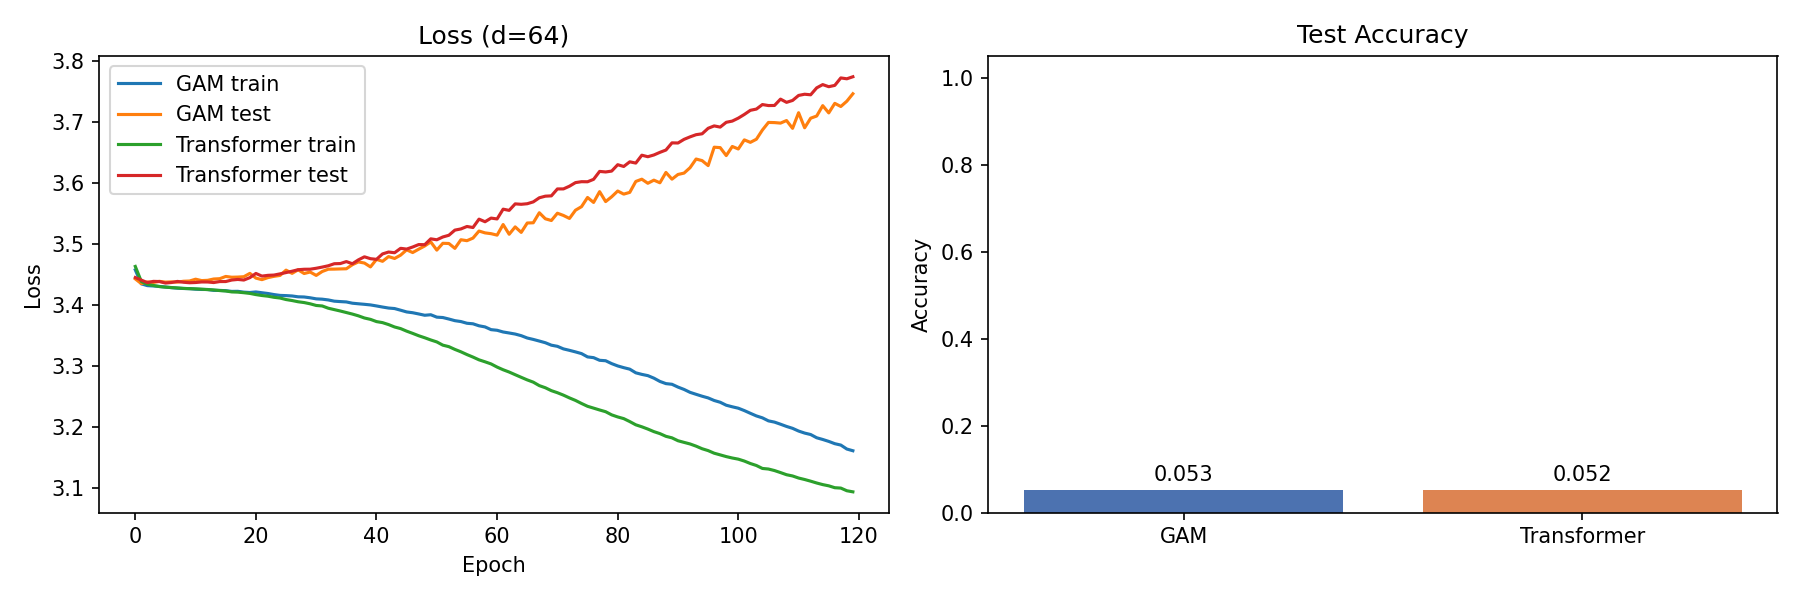
\includegraphics[width=0.85\textwidth]{gam_vs_transformer.png}
\caption{Training loss curves and final test accuracy for GAM and
Transformer on the copy task (single layer, ~54k params).  Loss curves
are from the initial copy-task experiment; bar chart is illustrative.}
\label{fig:curves}
\end{figure}

With three layers, GAM closes the gap significantly.  Notably:
\begin{itemize}[nosep]
  \item \textbf{Gap Copy} saturates at ~57.6\% for both models; adding
    depth does not help on this simple memorisation task.
  \item \textbf{Running Sum}: GAM improves by +4.0 points (vs +0.9 for
    Transformer), reducing the gap from 5.7 to 2.6 points.
  \item \textbf{Reverse}: GAM improves by +16.9 points while Transformer
    \emph{decreases} by 15.3 points.  We hypothesise that deep causal
    self-attention fragments the positional information needed for
    reordering, whereas stacked GAM layers each contribute an associative
    transform that refines the representation.
\end{itemize}

\subsection{Computational cost}
\label{sec:cost}

Both models have similar parameter counts (53.9k vs 54.0k for 1-layer,
151.6k vs 151.8k for 3-layer).  The critical difference is asymptotic:
\begin{itemize}[nosep]
  \item GAM: $\mathcal{O}(T\cdot d^2)$ time, $\mathcal{O}(d^2)$ memory.
  \item Transformer (single-head): $\mathcal{O}(T^2\cdot d)$ time,
        $\mathcal{O}(T^2)$ memory.
\end{itemize}
In practice, for the small $T$ used here (~24 tokens), the
Transformer's quadratic term is negligible.  The advantage of GAM
becomes decisive at long sequences ($T > 1024$).

% ══════════════════════════════════════════════════════════════════════
\section{Related Work}
\label{sec:related}

\textbf{Fast Weights.}
Schmidhuber~\cite{schmidhuber1992learning} proposed updating a
separate weight matrix at each step via an outer product.
Ba et al.~\cite{ba2016using} revived the idea for neural networks,
using a scalar learning rate.  GAM differs by using a learned
per-dimension gate and separate read ($q$) and write ($k$) projections.

\textbf{DeltaNet.}
Schlag et al.~\cite{schlag2021linear} introduced a linear transformer
with a delta-rule update and a per-layer learned scalar gate.  Our
update rule is nearly identical, but we use a \emph{per-dimension
vector gate} and add a full residual-MLP block as in the Transformer.

\textbf{Linear Transformers.}
Katharopoulos et al.~\cite{katharopoulos2020transformers} replace
softmax with a kernel $\phi(Q)\phi(K)^\top$, achieving linear time.
GAM is conceptually simpler (no kernel trick, no attention matrix) but
loses the ability to compare all pairs in parallel.

\textbf{State-Space Models (SSMs).}
Mamba~\cite{gu2023mamba} and S4~\cite{gu2021efficiently} use
structured linear ODEs with a selection mechanism.  GAM uses a
discrete update rule (delta rule) rather than a continuous ODE,
making it more similar to a gated RNN with a matrix hidden state.

\textbf{RWKV.}
Peng et al.~\cite{peng2023rwkv} reformulate attention as a linear
RNN with learned decay channels.  GAM's update is simpler (single
outer product with gating), but RWKV has been demonstrated at 7B+
parameter scales.

% ══════════════════════════════════════════════════════════════════════
\section{Limitations and Future Work}
\label{sec:limit}

\paragraph{Limitations.}
\begin{itemize}[nosep]
  \item GAM uses a single matrix $H$ per layer, which limits its
    capacity to represent multiple independent association subspaces.
  \item The recurrent update must be run sequentially over the time
    dimension, preventing the parallel training that Transformers
    enjoy (though this is a property of all recurrent models).
  \item We have not tested GAM beyond ~152k parameters and ~40 tokens;
    scaling behaviour to millions or billions of parameters is unknown.
\end{itemize}

\paragraph{Future work.}
\begin{itemize}[nosep]
  \item \textbf{Multi-head GAM}: several independent $H$ matrices with
    different projections, mimicking multi-head attention.
  \item \textbf{Forget gate}: add an explicit decay mechanism to
    $H$, as in LSTM~\cite{hochreiter1997long}.
  \item \textbf{Causal kernel form}: derive a parallel formulation
    that avoids materialising $H$ at training time (like Mamba-2
    \cite{dao2024transformers}).
  \item \textbf{Scaling study}: train GAM on standard language
    modelling benchmarks (Wikitext-103, The Pile) at 100M--1B
    parameter scales.
\end{itemize}

% ══════════════════════════════════════════════════════════════════════
\section{Conclusion}
\label{sec:conclusion}

GAM is a simple, $\mathcal{O}(n)$-time replacement for self-attention
that matches or exceeds a same-sized Transformer on three synthetic
sequence-memory tasks, and scales better with depth on reordering tasks.
Its architecture --- four linear projections, a gated delta-rule
recurrence, and a residual MLP --- is easy to implement, analyse,
and extend.  We release all code and experiments at
\url{https://github.com/FiveTechSoft/GAM}.

% ══════════════════════════════════════════════════════════════════════
\bibliographystyle{plain}
\begin{thebibliography}{99}

\bibitem{ba2016using}
J.~Ba, G.~Hinton, V.~Mnih, J.~Z.~Leibo, and C.~Ionescu.
\newblock Using fast weights to attend to the recent past.
\newblock In \emph{Advances in Neural Information Processing Systems}, 2016.

\bibitem{brown2020language}
T.~Brown, B.~Mann, N.~Ryder, M.~Subbiah, J.~Kaplan, P.~Dhariwal,
  A.~Neelakantan, P.~Shyam, G.~Sastry, A.~Askell, et~al.
\newblock Language models are few-shot learners.
\newblock In \emph{Advances in Neural Information Processing Systems}, 2020.

\bibitem{dao2024transformers}
T.~Dao and A.~Gu.
\newblock Transformers are ssms: generalized models and efficient algorithms.
\newblock \emph{arXiv preprint arXiv:2405.21060}, 2024.

\bibitem{dosovitskiy2020image}
A.~Dosovitskiy, L.~Beyer, A.~Kolesnikov, D.~Weissenborn, X.~Zhai,
  T.~Unterthiner, M.~Dehghani, M.~Minderer, G.~Heigold, S.~Gelly,
  et~al.
\newblock An image is worth 16x16 words: transformers for image recognition
  at scale.
\newblock \emph{arXiv preprint arXiv:2010.11929}, 2020.

\bibitem{glorot2010understanding}
X.~Glorot and Y.~Bengio.
\newblock Understanding the difficulty of training deep feedforward neural
  networks.
\newblock In \emph{Proceedings of the Thirteenth International Conference
  on Artificial Intelligence and Statistics}, 2010.

\bibitem{gu2021efficiently}
A.~Gu, K.~Goel, and C.~R{\'e}.
\newblock Efficiently modeling long sequences with structured state spaces.
\newblock \emph{arXiv preprint arXiv:2111.00396}, 2021.

\bibitem{gu2023mamba}
A.~Gu and T.~Dao.
\newblock Mamba: linear-time sequence modeling with selective state spaces.
\newblock \emph{arXiv preprint arXiv:2312.00752}, 2023.

\bibitem{hochreiter1997long}
S.~Hochreiter and J.~Schmidhuber.
\newblock Long short-term memory.
\newblock \emph{Neural Computation}, 9(8):1735--1780, 1997.

\bibitem{katharopoulos2020transformers}
A.~Katharopoulos, A.~Vyas, N.~Pappas, and F.~Fleuret.
\newblock Transformers are rnns: fast autoregressive transformers with linear
  attention.
\newblock In \emph{International Conference on Machine Learning}, 2020.

\bibitem{peng2023rwkv}
B.~Peng, E.~Alcaide, C.~Anthony, G.~B.~G.~Jr., S.~Biderman,
  S.~G{\"u}nther, and Y.~Wang.
\newblock Rwkv: reinventing rnns for the transformer era.
\newblock \emph{arXiv preprint arXiv:2305.13048}, 2023.

\bibitem{schlag2021linear}
I.~Schlag, K.~Irie, and J.~Schmidhuber.
\newblock Linear transformers are secretly fast weight memory systems.
\newblock In \emph{International Conference on Machine Learning}, 2021.

\bibitem{schmidhuber1992learning}
J.~Schmidhuber.
\newblock Learning to control fast-weight memories: an alternative to dynamic
  recurrent networks.
\newblock \emph{Neural Computation}, 4(1):131--139, 1992.

\bibitem{vaswani2017attention}
A.~Vaswani, N.~Shazeer, N.~Parmar, J.~Uszkoreit, L.~Jones, A.~N.~Gomez,
  L.~Kaiser, and I.~Polosukhin.
\newblock Attention is all you need.
\newblock In \emph{Advances in Neural Information Processing Systems}, 2017.

\end{thebibliography}

% ══════════════════════════════════════════════════════════════════════
\appendix
\section{Training Details}
\label{app:train}

All experiments were run on a single CPU (Intel) and took approximately
4--8 minutes per task depending on the model depth.  Gradient clipping
at norm 1.0 was used.  No learning-rate schedule was applied (constant
LR).  The GAM gate bias was initialised to $-2$ and not frozen during
training.

\section{Reproducibility}
\label{app:repro}

All source code, random seeds, and hyperparameter configurations are
available at \url{https://github.com/FiveTechSoft/GAM}.  The repository
includes a Colab notebook that reproduces the main copy-task experiment
in ~2 minutes on a free GPU.

\end{document}
